\documentclass[11pt]{amsart}
\usepackage{amssymb}
\usepackage{amsmath}
\usepackage{latexsym}
\usepackage{tikz}
\usepackage{hyperref}
\hypersetup{colorlinks=true,citecolor=blue,linkcolor=blue}

%\usepackage[margin=1in]{geometry}

% add yourself here in order to make comments on the side
\usepackage[draft]{say}
\newcommand{\sayDR}[1]{\say[DR]{#1}}
\newcommand{\saySS}[1]{\say[SS]{#1}}
\newcommand{\sayMC}[1]{\say[MC]{#1}}
\newcommand{\sayMG}[1]{\say[MG]{#1}}

% ambients
\newtheorem{lemma}{Lemma}[section]
\newtheorem{theorem}{Theorem}[section]
\newtheorem{propo}[theorem]{Proposition}
\newtheorem{prop}[theorem]{Proposition}
\newtheorem{cor}[theorem]{Corollary}
\newtheorem{conj}[theorem]{Conjecture}
\newtheorem{claim}[theorem]{Claim}
\newtheorem{claim*}{Claim}
\newtheorem{rmk}[theorem]{Remark}
\newtheorem{thm}[theorem]{Theorem}
\newtheorem{defn}[theorem]{Definition}
\theoremstyle{remark}
\newtheorem{example}[theorem]{Example}
\newtheorem{remark}[theorem]{Remark}
\newtheorem{question}[theorem]{Question}
\numberwithin{equation}{section}

% shorthands
\newcommand{\NN}{\mathbb{N}}
\newcommand{\QQ}{\mathbb{Q}}
\newcommand{\RR}{\mathbb{R}}
\newcommand{\ZZ}{\mathbb{Z}}

\newcommand{\cA}{\mathcal{A}}

\newcommand{\fd}{\mathfrak{d}}
\newcommand{\fD}{\mathfrak{D}}
\newcommand{\fm}{\mathfrak{m}}

\newcommand{\gr}{\mathrm{gr}}

\newcommand{\Hom}{\operatorname{Hom}}
\newcommand{\Mono}{\operatorname{Mono}}
\newcommand{\Spec}{\operatorname{Spec}}

%%%%%%%%%%%%%%%%%%%%%%%%%%%%%%%%%%%%%%%%%%%%%%%%%%%%%%%%%%%%%%%%%%%
\title[Greedy Basis is the Theta Basis]{A Rank Two Haiku:\\ The Greedy Basis Equals \\ The Theta Basis}
\author{CCGMMRSW}

\begin{document}
\maketitle

\begin{abstract}
We prove the equality of two canonical bases of a rank 2 cluster algebra, the greedy basis of Lee-Li-Zelevinsky and the theta basis of Gross-Hacking-Keel-Kontsevich.
\end{abstract}

\section{Introduction}

Cluster algebras are commutative rings with partial bases of a special form, originally discovered in the context of dual canonical bases in Lie theory.  Their axiomatics encapsulates the fact that many kinds of canonical bases in nature have large subsets which are governed by a uniform combinatorics.  Elements of these subsets are monomials in distinguished elements called cluster variables, which are grouped into overlapping collections called clusters.  Each cluster has an associated skew-symmetrizable matrix, and the entire cluster algebra can be reconstructed recursively from any particular cluster along with this matrix.

A fundamental issue in the theory is understanding natural completions of the partial basis of cluster monomials to a complete basis of a cluster algebra.  Depending on the context, this question can be analyzed from a wide range of perspectives drawn from representation theory, geometry, combinatorics, and mathematical physics \cite{???}.  Generally one expects any cluster algebra to admit several natural bases related in potentially subtle ways.  A basic example of this is the relationship between the dual canonical and dual semicanonical bases of the coordinate ring of the positive unipotent subgroup of a simple algebraic group \cite{???}.  This example illustrates in particular that in general it is nontrivial to tell even whether or not two constructions of canonical bases in a cluster algebra lead to the same result.  The purpose of the present paper is to compare two such constructions for cluster algebras associated to skew-symmetrizable matrices of rank 2.  

The first basis we consider is the greedy basis of \cite{LLZ}.  Every cluster algebra is contained in the ring of Laurent polynomials in the cluster variables of any of its clusters.  The recently-confirmed positivty conjecture asserts that the coefficients of these polynomials are positive integers.  The definition of the greedy basis builds this property into any canonical basis element by attempting to describe the minimal conditions for a Laurent polynomial in an initial cluster to be both positive and Laurent in the two adjacent clusters.  The resulting coefficients turn out to enumerate combinatorial objects called compatible pairs related to maximal Dyck paths.  

The second basis we consider is the theta basis of Gross-Hacking-Keel-Kontsevich \cite{GHKK}.  Unlike the greedy basis it is defined for cluster algebras of arbitrary rank.  The coefficients of Laurent expansions of its elements enumerate combinatorial objects called broken lines, which morally capture the geometry of holomorphic disks in the mirror cluster variety.  Broken lines are piecewise-linear paths in a tropicalization of the cluster variety, whose points of non-linearity lie along an object known as a scattering diagram.  This diagram encodes the relations among cluster transformations, or among elements of the tropical vertex group.

\begin{theorem}
Let $\mathcal{A}$ be a rank 2 cluster algebra.  The greedy and theta bases of $\mathcal{A}$ coincide.
\end{theorem}

The proof is based on an analysis of the Newton polygons of elements of the theta basis.  It can be shown that elements of the greedy basis are essentially determined by which coefficients of their Laurent expansion are nonzero.  That is, if an element of $\mathcal{A}$ is positive and Laurent in three adjacent clusters and has the same nonzero coefficients as a greedy basis element in any particular Laurent expansion, it must in fact coincide with that element.  Thus to show that elements of the theta basis are elements of the greedy basis, it suffices to establish certain bounds on the behavior of broken lines rather than explicitly enumerating them.

\textsc{Acknowledgements} This paper is the result of a working group on scattering diagrams at the 2014 AMS Mathematics Research Community on Cluster Algebras in Snowbird, UT, which explains the large number of authors.  We thank the AMS and in particular Ellen Maycock and Donna Salter for helping facilitate such an enjoyable and productive environment.  We also thank the other organizers Gordana Todorov, Michael Gekhtman, and David Speyer for making the workshop possible.

\section{Rank 2 cluster algebras and their greedy bases}
\saySS{This section was written by Dylan independently while Mark, Mandy and
  myself were working on sections 2 and 3. We should check that notations and
  conventions are consistent. I am ready to bet that we need to take a transpose somewhere.}\sayDR{Done, the conventions for mutations match.}
Fix $b,c>0$ and consider rational functions $x_m\in\QQ(x_1,x_2)$, for $m\in\ZZ$,
defined recursively by 
\[
  x_{m-1}x_{m+1}=
  \begin{cases}
    x_m^b+1 & \text{if $m$ is odd;}\\
    x_m^c+1 & \text{if $m$ is even.}
  \end{cases}
\] 
These functions are called \emph{cluster variables} and the \emph{cluster
algebra} $\cA(b,c)$ is the $\ZZ$-subalgebra of $\QQ(x_1,x_2)$ which they
generate.  While the cluster variables appear to be rational functions, it is a
remarkable fact that cancellations inevitably occur and one always obtains
Laurent expressions.  This result is known as the ``Laurent Phenomenon" and was
proven by Fomin and Zelevinsky.
\begin{theorem}\label{th:Laurent}\cite[Theorem~3.1]{FZ} 
  For any $k,m\in\ZZ$ we have $x_m\in\ZZ[x_k^{\pm1},x_{k+1}^{\pm1}]$.
\end{theorem}
\sayDR{In fact, they made the stronger conjecture that all of these Laurent
  expressions have positive coefficients.}

An element $x\in\ZZ[x_1^{\pm1},x_2^{\pm1}]$ is called \emph{pointed at
$(a_1,a_2)\in\ZZ^2$} if it can be written in the form
\[
  x=x_1^{-a_1}x_2^{-a_2}\sum\limits_{p,q\ge0}c(p,q)x_1^{bp}x_2^{cq},
\]
where $c(p,q)\in\ZZ$ with $c(0,0)=1$.  We will call such an $x$ \emph{positive
in the first cluster} if $c(p,q)\ge0$ for all $p,q\ge0$.  An element $x\in\cA(b,c)$ is simply called \emph{positive} if its Laurent expansion in each $\ZZ[x_k^{\pm1},x_{k+1}^{\pm1}]$ has positive coefficients.
\begin{prop}\cite[Proposition~1.5]{LLZ}
  Let $x$ be pointed at $(a_1,a_2)\in\ZZ^2$ and suppose
  $x\in\ZZ_{\ge0}[x_0^{\pm1},x_1^{\pm1}]
  \cap\ZZ_{\ge0}[x_1^{\pm1},x_2^{\pm1}]
  \cap\ZZ_{\ge0}[x_2^{\pm1},x_3^{\pm1}]$.
  Then the pointed coefficients $c(p,q)$ satisfy the following recursive
  inequality:
  \begin{align}
    \label{eq:consecutive positivity inequality}
    c(p,q)\ge\max\bigg(
    &\sum\limits_{k=1}^p (-1)^{k-1}c(p-k,q){a_2-cq+k-1\choose k}\\
    \nonumber&\sum\limits_{\ell=1}^q (-1)^{\ell-1}c(p,q-\ell){a_1-bp+\ell-1\choose \ell}\bigg).
  \end{align}
\end{prop}
A positive element $x\in\cA(b,c)$ is called \emph{indecomposable} if it cannot
be written as a sum of two positive elements.  In the search for positive bases
of $\cA(b,c)$ one is naturally led to investigate the indecomposable positive
elements.  A sufficient condition for a positive pointed element $x$ to be
indecomposable is the inequality \eqref{eq:consecutive positivity inequality}
being an equality.  It turns out that this requirement alone uniquely determines
a collection of elements of $\cA(b,c)$ with nice properties.

\begin{theorem}\label{th:greedy}\cite[Theorem~1.7]{LLZ}
  For any $(a_1,a_2)\in\ZZ^2$ there exists a unique indecomposable positive
  element $x[a_1,a_2]\in\cA(b,c)$ which is pointed at $(a_1,a_2)$ and whose
  pointed coefficients satisfy the recursion
  \begin{align}
    \label{eq:greey recursion}
    c(p,q)=\max\bigg(
    &\sum\limits_{k=1}^p (-1)^{k-1}c(p-k,q){a_2-cq+k-1\choose k}\\
    \nonumber&\sum\limits_{\ell=1}^q (-1)^{\ell-1}c(p,q-\ell){a_1-bp+\ell-1\choose \ell}\bigg).
  \end{align}
  Moreover, the collection $\{x[a_1,a_2]:(a_1,a_2)\in\ZZ^2\}$ is a basis of
  $\cA(b,c)$ which contains the cluster monomials and is independent of the
  choice of an initial cluster.
\end{theorem}
We will call $x[a_1,a_2]$ the \emph{greedy element} pointed at $(a_1,a_2)$ and
call $\{x[a_1,a_2]:(a_1,a_2)\in\ZZ^2\}$ the \emph{greedy basis} of $\cA(b,c)$.  Let
$R_{a_1,a_2}=\{(p,q)\in\ZZ_{\ge0}^2:c(p,q)\ne0 \text{ in } x[a_1,a_2]\}$ denote
the \emph{pointed support} of $x[a_1,a_2]$.  Theorem~\ref{th:greedy} is proven using the following characterization of the greedy elements by their
pointed supports.

\begin{theorem}\label{th:pointed supports}(\cite[Proposition~4.1]{LLZ} and \cite[Corollary 3.5]{LLZ2})
  For $(a_1,a_2)\in\ZZ^2$, the pointed support of $x[a_1,a_2]$ is determined as follows.
\begin{enumerate}
  \item If $a_1 \leq 0$ and $a_2 \leq 0$, then $R_{a_1,a_2} = \{(0,0)\}$.
  \item If $a_1 \leq 0 < a_2$, then $R_{a_1,a_2} = \{(p,0): 0 \leq p \leq a_2\}$.
  \item If $a_2 \leq 0 < a_1$, then $R_{a_1,a_2} = \{(0,q): 0 \leq q \leq a_1\}$.
  \item If $0<ba_2\leq a_1$, then $R_{a_1,a_2}=\left\{(p,q)\in\ZZ_{\ge0}^2\big|\; p\le a_{2},\; q\le a_{1}-bp\right\}$.
  \item If $0<ca_1\leq a_2$, then $R_{a_1,a_2}=\left\{(p,q)\in\ZZ_{\ge0}^2\big|\; q\le a_{1},\; p\le a_{2}-cq\right\}$.
  \item If $0 < a_1 < ba_2$ and $0 < a_2 < ca_1$, then
  $$\aligned
  R_{a_1,a_2}=&\bigg\{(p,q)\in\ZZ_{\ge0}^2\bigg|\; 0\le p< \frac{a_1}{b},\; q+\Big(b-\frac{ba_2}{ca_1}\Big)p<a_1\bigg\}\\
  &\bigcup\bigg\{(p,q)\in\ZZ_{\ge0}^2\bigg|\; 0\le q<
    \frac{a_2}{c},\; p+\Big(c-\frac{ca_1}{ba_2}\Big)q<a_2\bigg\}\\
  &\hspace{1.35em}\bigcup\Big\{(0,a_1),(a_2,0)\Big\}.
  \endaligned
  $$
\end{enumerate}
Moreover, if $x\in\cA(b,c)$ is any positive element pointed at $(a_1,a_2)$ whose pointed support is equal to $R_{a_1,a_2}$, then $x=x[a_1,a_2]$. 
\end{theorem}
\begin{proof}
 The first part is the content of \cite[Proposition~4.1]{LLZ} and \cite[Corollary 3.5]{LLZ2}.  Suppose $x\in\cA(b,c)$ is a positive element pointed at $(a_1,a_2)$ and the pointed support of $x$ is equal to $R_{a_1,a_2}$.  If $x$ is indecomposable, then we must have $x=x[a_1,a_2]$.  So suppose 
\end{proof}

\begin{remark}
  Consider the points 
  \[
    O=(0,0), \quad A=(-a_1+ba_2,0), \quad B=(-a_1,-a_2), \quad C=(-a_1,-a_2+ca_1),
  \]
  \[
    D_{1}=(-a_1+ba_{2},ca_{1}-(bc+1)a_{2}), \quad D_{2}=(ba_{2}-(bc+1)a_{1},-a_2+ca_{1}).
  \]  
  Then the Newton polytope of $x[a_1,a_2]$ can be visualized as in Figure~\ref{fig:greedy polytopes}.
  \begin{figure}
    \centering
    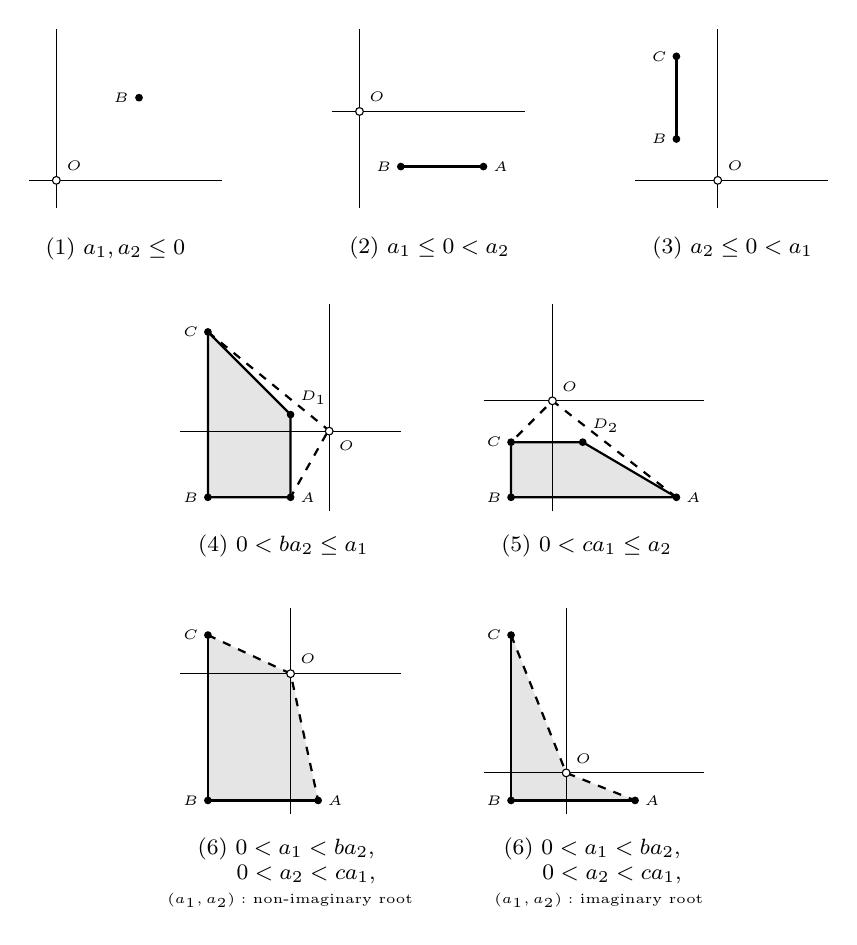
\begin{tikzpicture}[scale=.7]
      %(1)
      \begin{scope}[shift={(-2.75, 5.5)}]
        \usetikzlibrary{patterns}
        \draw[-] (-0.5,0.25) -- (3,0.25);
        \draw[-] (0,-0.25) -- (0,3);
        \fill[white] (0,0.25) circle (2pt);
        \draw (0,0.25) circle (2pt);
        \draw (0,0.25) node[anchor=south west] {\tiny $O$};
        \fill (1.5,1.75) circle (2pt);
        \draw (1.5,1.75) node[anchor=east] {\tiny $B$};
        \draw (1.07,-.6) node[anchor=north] {\footnotesize (1) $a_1,a_2\le0$};
      \end{scope}
      %(2)
      \begin{scope}[shift={(2.75, 5.5)}]
        \usetikzlibrary{patterns}
        \draw[-] (-0.5,1.5) -- (3,1.5);
        \draw[-] (0,-0.25) -- (0,3);
        \fill[white] (0,1.5) circle (2pt);
        \draw (0,1.5) circle (2pt);
        \draw (0,1.5) node[anchor=south west] {\tiny $O$};
        \fill (2.25,0.5) circle (2pt);
        \draw (2.25,0.5) node[anchor=west] {\tiny$A$};
        \fill (0.75,0.5) circle (2pt);
        \draw (0.75,0.5) node[anchor=east] {\tiny$B$};
        \draw [thick] (0.75,0.5) -- (2.25,0.5);
        \draw (1.27,-.6) node[anchor=north] {\footnotesize (2) $a_1\le 0<a_2$};
      \end{scope}
      %(3)
      \begin{scope}[shift={(8.25,5.5)}]
        \usetikzlibrary{patterns}
        \draw [thick] (0.25,1) -- (0.25,2.5);
        \draw[-] (-0.5,0.25) -- (3,0.25);
        \draw[-] (1,-0.25) -- (1,3);
        \fill[white] (1,0.25) circle (2pt);
        \draw (1,0.25) circle (2pt);
        \draw (1,0.25) node[anchor=south west] {\tiny $O$};
        \fill (0.25,1) circle (2pt);
        \draw (0.25,1) node[anchor=east] {\tiny$B$};
        \fill (0.25,2.5) circle (2pt);
        \draw (0.25,2.5) node[anchor=east] {\tiny$C$};
        \draw (1.27,-.6) node[anchor=north] {\footnotesize (3) $a_2\le0<a_1$};
      \end{scope}
      %(4)
      \begin{scope}[shift={(0,0)}]
        \usetikzlibrary{patterns}
        %\fill[pattern=horizontal lines] (-2.5,2)--(-1,.5)--(-1,-1)--(-2.5,-1)--(-2.5,2);
        \fill[black!10] (0,3)--(1.5,1.5)--(1.5,0)--(0,0)--(0,3);
        \draw[thick] (0,3)--(1.5,1.5)--(1.5,0)--(0,0)--(0,3);
        \draw[dashed,thick](0,3)--(2.15,1.25) (2.15,1.15)--(1.5,0);
        \draw[-] (-0.5,1.2) -- (3.5,1.2);
        \draw[-] (2.2,-0.25) -- (2.2,3.5);
        \fill[white] (2.2,1.2) circle (2pt);
        \draw (2.2,1.2) circle (2pt);
        \draw (2.2,1.2) node[anchor=north west] {\tiny$O$};
        \fill (1.5,0) circle (2pt);
        \draw (1.5,0) node[anchor=west] {\tiny$A$};
        \fill (0,0) circle (2pt);
        \draw (0,0) node[anchor=east] {\tiny$B$};
        \fill (0,3) circle (2pt);
        \draw (0,3) node[anchor=east] {\tiny$C$};
        \fill (1.5,1.5) circle (2pt);
        \draw (1.5,1.5) node[anchor= south west] {\tiny$D_{1}$};
        \draw (1.37,-0.5) node[anchor=north] {\footnotesize (4) $0<ba_2\leq a_1$};
      \end{scope}
      %(5)
      \begin{scope}[shift={(5.5,0)}]
        \usetikzlibrary{patterns}
        \fill[black!10] (3,0)--(1.3,1)--(0,1)--(0,0)--(3,0);
        \draw[thick] (3,0)--(1.3,1)--(0,1)--(0,0)--(3,0);
        \draw[dashed,thick](3,0)--(0.75,1.75)--(0,1);
        \draw[-] (-0.5,1.75) -- (3.5,1.75);
        \draw[-] (0.75,-0.25) -- (0.75,3.5);
        \fill[white] (0.75,1.75) circle (2pt);
        \draw (0.75,1.75) circle (2pt);
        \draw (0.75,1.75) node[anchor=south west] {\tiny$O$};
        \fill (3,0) circle (2pt);
        \draw (3,0) node[anchor=west] {\tiny$A$};
        \fill (0,0) circle (2pt);
        \draw (0,0) node[anchor=east] {\tiny$B$};
        \fill (0,1) circle (2pt);
        \draw (0,1) node[anchor=east] {\tiny$C$};
        \fill (1.3,1) circle (2pt);
        \draw (1.3,1) node[anchor=south west] {\tiny$D_{2}$};
        \draw (1.37,-.5) node[anchor=north] {\footnotesize (5) $0<ca_1\leq a_2$};
      \end{scope}
      %(6)
      \begin{scope}[shift={(0,-5.5)}]
        \usetikzlibrary{patterns}
        \fill[black!10]  (0,3)--(1.5,2.3)--(2,0)--(0,0)--(0,3);
        \draw[thick] (0,3)--(0,0)--(2,0); 
        \draw[dashed,thick] (0,3)--(1.5,2.3)--(2,0);
        \draw[-] (-0.5,2.3) -- (3.5,2.3);
        \draw[-] (1.5,-0.25) -- (1.5,3.5);
        \fill[white] (1.5,2.3) circle (2pt);
        \draw (1.5,2.3) circle (2pt);
        \draw (1.5,2.3) node[anchor=south west] {\tiny$O$};
        \fill (2,0) circle (2pt);
        \draw (2,0) node[anchor=west] {\tiny$A$};
        \fill (0,0) circle (2pt);
        \draw (0,0) node[anchor=east] {\tiny$B$};
        \fill (0,3) circle (2pt);
        \draw (0,3) node[anchor=east] {\tiny$C$};
        \draw (1.42,-.5) node[anchor=north] {\footnotesize (6) $0<a_1<ba_2$,};
        \draw (1.46,-1) node[anchor=north] {\footnotesize \hspace{10pt} $0<a_2<ca_1$,};
        \draw (1.17,-1.5) node[anchor=north] {\footnotesize \hspace{10pt} \tiny{$(a_1,a_2):$ non-imaginary root}};
      \end{scope}
      %(6')
      \begin{scope}[shift={(5.5,-5.5)}]
        \usetikzlibrary{patterns}
        \fill[black!10]  (0,3)--(1,0.5)--(2.25,0)--(0,0)--(0,3);
        \draw[thick] (0,3)--(0,0)--(2.25,0);
        \draw[dashed,thick] (0,3)--(1,0.5)--(2.25,0);
        \draw[-] (-0.5,0.5) -- (3.5,0.5);
        \draw[-] (1,-0.25) -- (1,3.5);
        \fill[white] (1,0.5) circle (2pt);
        \draw (1,0.5) circle (2pt);
        \draw (1,0.5) node[anchor=south west] {\tiny$O$};
        \fill (2.25,0) circle (2pt);
        \draw (2.25,0) node[anchor=west] {\tiny$A$};
        \fill (0,0) circle (2pt);
        \draw (0,0) node[anchor=east] {\tiny$B$};
        \fill (0,3) circle (2pt);
        \draw (0,3) node[anchor=east] {\tiny$C$};
        \draw (1.47,-.5) node[anchor=north] {\footnotesize (6) $0<a_1<ba_2$,};
        \draw (1.51,-1) node[anchor=north] {\footnotesize \hspace{10pt} $0<a_2<ca_1$,};
        \draw (1.27,-1.5) node[anchor=north] {\footnotesize \hspace{10pt} \tiny{$(a_1,a_2):$ imaginary root}};
      \end{scope}
    \end{tikzpicture}
    \caption{The Newton polytope of $x[a_1,a_2]$.} 
    \label{fig:greedy polytopes}
  \end{figure}
\end{remark}

To prove Theorem~\ref{th:pointed supports} Lee, Li, and Zelevinsky develop a
combinatorial construction via compatible pairs on a maximal Dyck path.  

For $(a_1,a_2)\in\ZZ_{\ge0}^2$, a Dyck path in the rectangle
$[0,a_1]\times[0,a_2]$ is a lattice path beginning at $(0,0)$ which takes steps
to the east and north to end at $(a_1,a_2)$ while never crossing above the main
diagonal.  Let $D_{a_1,a_2}$ denote the maximal such Dyck path, i.e. any lattice
point lying strictly above the Dyck path $D_{a_1,a_2}$ also lies above the main
diagonal.  

Let $H$ and $V$ denote the sets of horizontal and vertical edges of
$D_{a_1,a_2}$.  For edges $e_1,e_2\in D_{a_1,a_2}$ write $e_1e_2$ for the
subpath of $D_{a_1,a_2}$ which begins at $e_1$ and terminates at $e_2$.  When
$e_1$ comes after $e_2$ the path $e_1e_2$ begins at $e_1$ goes to the end of
$D_{a_1,a_2}$ and then continues from the beginning of $D_{a_1,a_2}$ to $e_2$.
Write $(e_1e_2)_H$ and $(e_1e_2)_V$ for the sets of horizontal and vertical
edges in $e_1e_2$.

For $S_1\subset H$ and $S_2\subset V$ we call the pair $(S_1,S_2)$
\emph{compatible} if for each $h\in S_1$ and $v\in S_2$ there exists an edge
$e\in hv$ such that one of the following holds:
\begin{align*}
 \tag{HSC}\label{eq:horizontal shadow condition}\big|(he)_V\big|=b\big|(he)_H\cap S_1\big|\quad&\text{and}\quad e\ne v;\\
 \tag{VSC}\label{eq:vertical shadow condition}\big|(ev)_H\big|=c\big|(ev)_V\cap S_2\big|\quad&\text{and}\quad e\ne h.\\
\end{align*}
We call the first the ``horizontal shadow condition" and call the second the
``vertical shadow condition".
\begin{theorem}
  \label{th:combinatorial greedy}\cite[Theorem~1.11]{LLZ}
  For any $(a_1,a_2)\in\ZZ^2$ we have
  \begin{equation}
    \label{eq:combinatorial greedy}
    x[a_1,a_2]=x_1^{-a_1}x_2^{-a_2}\sum\limits_{(S_1,S_2)}x_1^{b|S_2|}x_2^{c|S_1|},
  \end{equation}
  where $(S_1,S_2)$ runs over all compatible pairs in the maximal Dyck path
  $D_{[a_1]_+,[a_2]_+}$.
\end{theorem}

\section{Scattering diagrams and broken lines}
\saySS{We are using Fock-Goncharov conventions through the paper; in particular
  we denote initial cluster variables by $A_i$ and we read mutations by rows.
  All the relevant notions, (in particular $d$- and $g$-vectors) are
  the ``transposed'' of those in Fomin-Zelevinsky and Lee-Li-Zelevinsky. We
  should mention these facts in the introduction.}
In this section, we will describe the cluster algebras $\cA (b,c)$ from the
point of view of scattering diagrams. While all the results in this section are
derived from \cite{GHKK}, we will adopt a slightly simplified notation here
sufficient for the rank $2$ case.

Let $N = \ZZ^2$ be a lattice and $M = \Hom (N, \ZZ)$. We will write elements of
$N$ and of $M$ both as tuples and, for $m\in N$, $n\in N$, we will denote their 
standard pairing by $n \cdot m$. Write
$M_{\RR} = M\otimes\RR$, $N_{\RR} = N\otimes\RR$. Take $\Bbbk$ to be a field of
characteristic 0.  For $m\in M$ we will write $A^m$ for the monomial in
$\Bbbk[M]$.  For notational convenience we will write $A_1=A^{(1,0)}$ and
$A_2=A^{(0,1)}$, thus we may identify $A^m$ with $A_1^{m_1}A_2^{m_2}$.

Let $\sigma \subsetneq M_{\RR}$ be a strictly convex rational cone; set
$P=\sigma \cap M$, and write $\widehat{\Bbbk[P]}$ for the completion of the
monoid ring $\Bbbk[P]$ at the maximal monomial ideal $\fm$ generated by
$\left\{A^m \,|\, m\in P\setminus\{0\}\right\}$.

\begin{defn}
  \label{walldef}
  A \emph{wall} is a pair $(\fd, f_{\fd})$, where 
  \begin{itemize}

    \item 
      $\fd \subset M_{\mathbb{R}}$ is either a ray $\RR_{\le 0} w$ or a line
      $\RR w$ with $w\in \sigma \cap(M\setminus 0)$;

    \item 
      $f_{\fd} \in \widehat{\Bbbk [P]}$ is such that 
      \[ 
        f_{\fd} = f_{\fd}(A^w) = 1 + \sum_{k\geq 1} c_k A^{k w},
      \] 
      for some $c_k \in \Bbbk$. 
  \end{itemize}
  The set $\fd \subset M_{\mathbb{R}}$ is called the \emph{support} of the wall
  $(\fd, f_{\fd})$.
\end{defn}

\begin{defn}
  \label{def:scattering_diagram}
  A scattering diagram $\fD$ is a collection of walls such that, for each $k \geq
  0$, the set
  \[
    \{ (\fd, f_{\fd}) \in \fD\, |\, f_{\fd} \neq 1 \bmod \fm^k \}
  \]
  is finite. %For semplicity we diverge slightly form the convention in
  %\cite{GHKK} by requiring that $\fd_1 \neq \fd_2$ whenever $f_{\fd_1}\neq
  %f_{\fd_2}$.
\end{defn}
For simplicity, we will impose the additional condition that $\fd_1\neq \fd_2$ for all pairs of walls in the scattering diagram.

For a scattering diagram $\fD$, we denote the support of $\fD$ as
\[
  \text{Supp} (\fD) := \bigcup_{(\fd, f_{\fd}) \in \fD} \fd. 
\]

To each wall $(\fd, f_{\fd})$, given a direction $v$ transversal to $\fd$, one
can associate the element $\theta_{v,\fd}\in
{\mathrm{Aut}}_{\Bbbk-alg}\left(\widehat{\Bbbk[P]}\right)$ defined by
\[
  \theta_{v,\fd} (A^m) := A^m f_{\fd}^{m\cdot n }, 
\]
where $n\in N$ is primitive, annihilates the tangent space to $\fd$, and is
uniquely determined by the sign convention $ v\cdot n <0$.  Note
that the only role of the transversal direction $v$ is to fix which of the two
normals $\pm n$ is used in the exponent. 

Consider a smooth immersion
\[  
  \gamma: [0,1] \rightarrow M_{\mathbb{R}} \backslash  \{0 \}  
\]
with endpoints not in the support of $\fD$. Assume $\gamma$ is transversal to
each wall of $\fD$ that it crosses. For each power $k \geq 1$, let  
\[
  0< t_1 <  t_2 < \cdots < t_s < 1 
\]
be the longest sequence of numbers such that $\gamma(t_i)\in\fd_i$ for some wall
$(\fd_i,f_{\fd_i}) \in \fD$ with $f_{\fd_i} \neq 1 \text{ mod } \fm^k$.

In view of the definition of scattering diagram, such a sequence is finite; we
can therefore consider the composition 
\[
  \theta^k_{\gamma, \fD} :=
  \theta_{\gamma'(t_s),\fd_s} \circ \cdots \circ \theta_{\gamma'(t_1),\fd_1}.
\]
Define the \textit{path-ordered product} along $\gamma$ as
\[
  \theta_{\gamma, \fD} := \lim_{k \rightarrow \infty} \theta ^k_{\gamma, \fD}. 
\]

\begin{defn}
  A scattering diagram is \emph{consistent} if $\theta _{\gamma, \fD}$ depends
  only on the endpoints of $\gamma$ for any path $\gamma$ for which
  $\theta_{\gamma, \fD}$ is well defined.
\end{defn}

\begin{theorem}[Kontsevich-Soibelman] 
  \label{KS}
  Given a scattering diagram $\fD$, there always exists a consistent scattering
  diagram $\fD'$ which contains $\fD$ such that $\fD'\setminus\fD$ only consists
  of rays.
\end{theorem}

We will now describe the scattering diagram $\fD_{(b,c)}$ associated to 
$\cA(b,c)$.
Recall that the initial exchange matrix in $\cA(b,c)$ is 
\[
  \epsilon = \begin{pmatrix} 0 & c\\ -b & 0\end{pmatrix},
\]
where $b$, $c$ are positive integers.  Following Example 1.30 of \cite{GHKK}, we
take $\sigma$ to be the second quadrant, i.e., the cone generated by $(-1,0)$ and
$(0,1)$. Then the ``initial'' scattering diagram associated to the above exchange
matrix is
\[
  \fD_{\mathrm{in},(b,c)} := 
  \left\{
    \big( \RR (-1,0), 1+A_1^{-b}\big), 
    \big( \RR (0,1), 1+A_2^c\big) 
  \right\}.
\]

We will denote by $\fD_{(b,c)}$ the consistent scattering diagram obtained by
applying Theorem \ref{KS} to $\fD_{\mathrm{in},(b,c)}$.

\begin{example} 
  \label{ex}
  Consider $\cA(2,1)$. Then we get
  \[
    \fD_{\mathrm{in},(2,1)} =  
    \left\{ 
      \big(\RR (-1,0), 1+A_1^{-2}\big), 
      \big(\RR (0,1), 1+A_2\big)  
    \right\}   
  \]
  and the associated consistent scattering diagram $\fD_{(2,1)}$ (shown in
  Figure~\ref{fig:diagex}) contains $\fD_{\mathrm{in},(2,1)}$ together with
  the two walls
  \[ 
    \big( \RR_{\leq 0} (-1,1), 1+A_1^{-2}A_2^2 \big)
    \quad \mbox{and} \quad
    \big( \RR_{\leq 0} (-2,1), 1+A_1^{-2}A_2 \big).
  \]
\end{example}

\begin{figure}
  \centering
  \begin{tikzpicture}
    \draw (3,0) -- (-3,0) node[left] {$1+A_1^{-2}$};
    \draw (0,-3) -- (0,3) node[above] {$1+A_2$};
    \draw (0,0) -- (3,-3) node[below right] {$1+A_1^{-2}A_2^2$};
    \draw (0,0) -- (3,-1.5) node[below right] {$1+A_1^{-2}A_2$};
  \end{tikzpicture}
  \caption{The scattering diagram $\fD_{(2,1)}$} 
  \label{fig:diagex}
\end{figure}

For general $b$ and $c$, the diagram $\fD_{(b,c)} \backslash
\fD_{\mathrm{in},(b,c)}$ may consist of an infinite number of rays, and in fact
it is infinite precisely when $bc\ge 4$. A more detailed description of the rays
which appear can be found in \cite{GHKK}, Example 1.30. We summarize the crucial
points here.

First of all note that, in view of the definition of scattering diagram, all the
rays in  $\fD_{(b,c)} \backslash \fD_{\mathrm{in},(b,c)}$ are contained in the
fourth quadrant.  To make our next observation we need to extend the action of
linear operators on $M_\RR$ to an action on pairs $(\fd,f_\fd)$. If $S$ is
linear on $M_\RR$ set
\begin{equation}
  \label{eqn:linear action}
  S(\fd,f_\fd(A^w))
  :=
  \left( S(\fd), f_\fd\left(A^{S(w)}\right) \right)
\end{equation}
Note that, even if $(\fd,f_\fd)$ is a wall, $S(\fd,f_\fd)$ needs not be a wall
since $S(w)$ may lay outside of the cone $\sigma$ (in which case we also get
that  $f_\fd\left(A^{S(w)}\right)$ is not an element of $\widehat{\Bbbk [P]}$).

Now consider the two linear involutions $S_1$ and $S_2$ given by
\[
  S_1 =  
  \begin{pmatrix}
    -1 & -b \\
    0& 1
  \end{pmatrix}
  %
  \quad
  \mbox{and}
  \quad
  %
  S_2 =  
  \begin{pmatrix}
    1 & 0 \\
    -c & -1
  \end{pmatrix}.
\]
If $(\fd, f_{\fd}) \in \fD_{(b,c)} \backslash \fD_{\mathrm{in},(b,c)}$ and $S_i
(\fd)$ is contained strictly in the fourth quadrant, then $S_i(\fd, f_{\fd}) \in
\fD_{(b,c)} \backslash \fD_{\mathrm{in},(b,c)}$. Moreover both 
\begin{equation}
  \label{eq:first-walls}
  S_2\big(\RR_{\leq 0}(-1,0),1+A_1^{-b}\big)
  %
  \quad
  \mbox{and}
  \quad
  %
  S_1\big(\RR_{\leq 0}(0,1),1+A_2^c\big)
\end{equation}
are walls in $\fD_{(b,c)} \backslash \fD_{\mathrm{in},(b,c)}$ even though
neither 
\[
  \big(\RR_{\leq 0}(-1,0),1+A_1^{-b}\big)
  %
  \quad
  \mbox{nor}
  \quad
  %
  \big(\RR_{\leq 0}(0,1),1+A_2^c\big)
\]
are walls in $\fD_{(b,c)}$. These considerations gives us a recipe to produce
elements of $\fD_{(b,c)} \backslash \fD_{\mathrm{in},(b,c)}$: it is enough to apply
alternatively $S_1$ and $S_2$ to the walls (\ref{eq:first-walls}).

We need to distinguish two cases. If $bc<4$ this procedure will construct, in
finitely many steps, all the walls in $\fD_{(b,c)} \backslash
\fD_{\mathrm{in},(b,c)}$.  If $bc\geq 4$, instead, we will get two infinite
families of walls whose supports will converge to the boundary of the convex cone
spanned by the irrational vectors
\[
  \left(2b,-bc + \sqrt{bc(bc-4)}\right)
  \quad
  \mbox{and}
  \quad
  \left(2b,-bc - \sqrt{bc(bc-4)}\right)
\]
These will exhaust all the walls in  $\fD_{(b,c)} \backslash \fD_{\mathrm{in},(b,c)}$
with support laying outside of this cone. The structure of the remaining part of 
$\fD_{(b,c)}$ is not completely understood; the expectation is that there is
a wall for each possible rational slope inside the irrational cone.
\sayMC{more detail at end?}
\sayMG{Wait and see what other facts we need about
  the diagram.} 

On the other hand the chamber structure one sees outside of the irrational cone
is very well-behaved and familiar in the theory of cluster algebras. This
chamber structure coincides with the Fock-Goncharov cluster complex, see
\cite{GHKK}, \S2, the mutation fan of Reading \cite{R}, and the picture group of
Igusa-Orr-Todorov-Weyman \cite{IOTW}.

\begin{figure}
  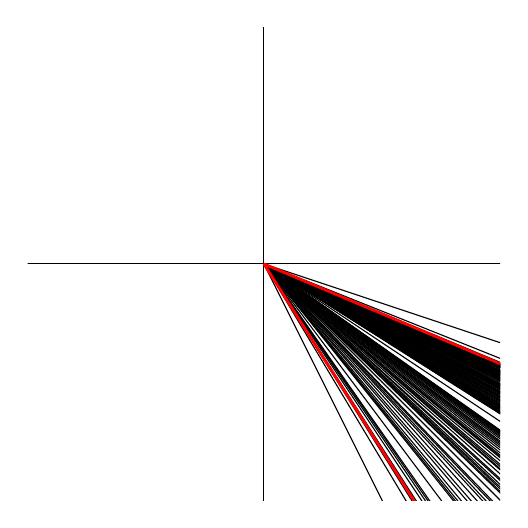
\begin{tikzpicture}[scale=0.1]
\clip (-30, -30) rectangle (30, 30);
\draw[color=black] (0,0) -- (-0.000000000000000, 60.0000000000000);
\draw[color=black] (0,0) -- (-60.0000000000000, -0.000000000000000);
\draw[color=black] (0,0) -- (-0.000000000000000, -60.0000000000000);
\draw[color=black] (0,0) -- (26.8328157299975, -53.6656314599950);
\draw[color=black] (0,0) -- (30.8697453256516, -51.4495755427527);
\draw[color=black] (0,0) -- (31.7999364001908, -50.8798982403053);
\draw[color=black] (0,0) -- (32.4454554788099, -50.4707085225932);
\draw[color=black] (0,0) -- (33.2820117735137, -49.9230176602706);
\draw[color=black] (0,0) -- (33.8002094784906, -49.5736405684529);
\draw[color=black] (0,0) -- (34.1525987298185, -49.3315314986267);
\draw[color=black] (0,0) -- (34.4077406617997, -49.1539152311424);
\draw[color=black] (0,0) -- (36.0000000000000, -48.0000000000000);
\draw[color=black] (0,0) -- (37.4817028532655, -46.8521285665818);
\draw[color=black] (0,0) -- (37.7002264252573, -46.6764708122233);
\draw[color=black] (0,0) -- (37.9942674154358, -46.4374379521993);
\draw[color=black] (0,0) -- (38.4110639798688, -46.0932767758426);
\draw[color=black] (0,0) -- (39.0474824073581, -45.5553961419178);
\draw[color=black] (0,0) -- (39.5102764721111, -45.1546016824127);
\draw[color=black] (0,0) -- (40.1378838973470, -44.5976487748300);
\draw[color=black] (0,0) -- (40.6968061639840, -44.0882066776493);
\draw[color=black] (0,0) -- (41.0364677328798, -43.7722322484051);
\draw[color=black] (0,0) -- (41.4285448009500, -43.4013326486143);
\draw[color=black] (0,0) -- (41.6481342350539, -43.1906577252411);
\draw[color=black] (0,0) -- (42.4264068711929, -42.4264068711929);
\draw[color=black] (0,0) -- (43.0740236070633, -41.7687501644250);
\draw[color=black] (0,0) -- (43.2192128094889, -41.6185012239522);
\draw[color=black] (0,0) -- (43.4482758620690, -41.3793103448276);
\draw[color=black] (0,0) -- (43.6207891529890, -41.1974119778230);
\draw[color=black] (0,0) -- (43.8633160945721, -40.9390950216007);
\draw[color=black] (0,0) -- (44.2292484120445, -40.5434777110408);
\draw[color=black] (0,0) -- (44.3964044037566, -40.3603676397788);
\draw[color=black] (0,0) -- (44.8445591210196, -39.8618303297952);
\draw[color=black] (0,0) -- (45.2263637944671, -39.4281120259456);
\draw[color=black] (0,0) -- (45.3413449673891, -39.2958323050705);
\draw[color=black] (0,0) -- (45.5553961419178, -39.0474824073581);
\draw[color=black] (0,0) -- (45.7505481223675, -38.8186468917058);
\draw[color=black] (0,0) -- (46.0932767758426, -38.4110639798688);
\draw[color=black] (0,0) -- (46.3844022289554, -38.0589967006814);
\draw[color=black] (0,0) -- (46.5140991310374, -37.9003770697341);
\draw[color=black] (0,0) -- (46.6346922424491, -37.7518937200779);
\draw[color=black] (0,0) -- (46.8521285665818, -37.4817028532655);
\draw[color=black] (0,0) -- (47.1295003336521, -37.1323335962108);
\draw[color=black] (0,0) -- (47.3611330425796, -36.8364368108952);
\draw[color=black] (0,0) -- (47.5574393462760, -36.5826456509815);
\draw[color=black] (0,0) -- (47.7259032019499, -36.3625929157714);
\draw[color=black] (0,0) -- (47.8720394353344, -36.1699853511415);
\draw[color=black] (0,0) -- (48.0000000000000, -36.0000000000000);
\draw[color=black] (0,0) -- (48.2134316006847, -35.7136530375442);
\draw[color=black] (0,0) -- (48.3842997513423, -35.4818198176510);
\draw[color=black] (0,0) -- (48.5241650581913, -35.2903018605028);
\draw[color=black] (0,0) -- (48.6407537039929, -35.1294332306615);
\draw[color=black] (0,0) -- (48.7394240154955, -34.9924069854839);
\draw[color=black] (0,0) -- (48.8240082724041, -34.8742916231458);
\draw[color=black] (0,0) -- (48.8973194741253, -34.7714271816002);
\draw[color=black] (0,0) -- (48.9614688660993, -34.6810404468203);
\draw[color=black] (0,0) -- (49.0180717958857, -34.6009918559193);
\draw[color=black] (0,0) -- (49.0683851580460, -34.5296043704768);
\draw[color=black] (0,0) -- (49.9230176602706, -33.2820117735137);
\draw[color=black] (0,0) -- (50.6527689148682, -32.1604881999163);
\draw[color=black] (0,0) -- (50.6891445332537, -32.1031248710607);
\draw[color=black] (0,0) -- (50.7293341818583, -32.0395794832789);
\draw[color=black] (0,0) -- (50.7739704053850, -31.9687961811684);
\draw[color=black] (0,0) -- (50.8238336704889, -31.8894642638361);
\draw[color=black] (0,0) -- (50.8798982403053, -31.7999364001908);
\draw[color=black] (0,0) -- (50.9433962264151, -31.6981132075472);
\draw[color=black] (0,0) -- (51.0159088012717, -31.5812768769777);
\draw[color=black] (0,0) -- (51.0994990022726, -31.4458455398601);
\draw[color=black] (0,0) -- (51.1969100191175, -31.2870005672385);
\draw[color=black] (0,0) -- (51.2519133368663, -31.1968168137447);
\draw[color=black] (0,0) -- (51.3118698932411, -31.0981029656007);
\draw[color=black] (0,0) -- (51.3774785130198, -30.9895902142024);
\draw[color=black] (0,0) -- (51.4495755427527, -30.8697453256516);
\draw[color=black] (0,0) -- (51.5291702980016, -30.7366980724922);
\draw[color=black] (0,0) -- (51.6174920180505, -30.5881434181040);
\draw[color=black] (0,0) -- (51.7160529094662, -30.4212075938036);
\draw[color=black] (0,0) -- (51.8267340539060, -30.2322615314452);
\draw[color=black] (0,0) -- (51.9084000879008, -30.0918261379135);
\draw[color=black] (0,0) -- (51.9519043946730, -30.0166558724777);
\draw[color=black] (0,0) -- (51.9973474124501, -29.9378666920167);
\draw[color=black] (0,0) -- (52.0945885274676, -29.7683363014100);
\draw[color=black] (0,0) -- (52.2013311509167, -29.5807543188528);
\draw[color=black] (0,0) -- (52.2587080645757, -29.4792712159145);
\draw[color=black] (0,0) -- (52.3190271231289, -29.3720854024583);
\draw[color=black] (0,0) -- (52.3503609569832, -29.3162021359106);
\draw[color=black] (0,0) -- (52.4494365672923, -29.1385758707179);
\draw[color=black] (0,0) -- (52.5568645648961, -28.9443601951602);
\draw[color=black] (0,0) -- (52.5947130467757, -28.8755287315631);
\draw[color=black] (0,0) -- (52.6257760704901, -28.8188773719351);
\draw[color=black] (0,0) -- (52.6737343748631, -28.7311278408344);
\draw[color=black] (0,0) -- (52.7234062015372, -28.6398749736745);
\draw[color=black] (0,0) -- (52.7575179922064, -28.5769889124452);
\draw[color=black] (0,0) -- (52.8013303601801, -28.4959560673988);
\draw[color=black] (0,0) -- (52.8282659953305, -28.4459893821010);
\draw[color=black] (0,0) -- (52.9411764705882, -28.2352941176471);
\draw[color=black] (0,0) -- (53.0420976185223, -28.0452470166899);
\draw[color=black] (0,0) -- (53.0630851708182, -28.0055171734874);
\draw[color=black] (0,0) -- (53.0950933429189, -27.9447859699573);
\draw[color=black] (0,0) -- (53.1498921168093, -27.8404196802335);
\draw[color=black] (0,0) -- (53.1950907699273, -27.7539604017012);
\draw[color=black] (0,0) -- (53.2652718869358, -27.6190298673000);
\draw[color=black] (0,0) -- (53.3172394232918, -27.5185751862151);
\draw[color=black] (0,0) -- (53.3384733855962, -27.4773953804586);
\draw[color=black] (0,0) -- (53.3890477687642, -27.3789988557765);
\draw[color=black] (0,0) -- (53.4260809317648, -27.3066635873465);
\draw[color=black] (0,0) -- (53.4543688141188, -27.2512468464135);
\draw[color=black] (0,0) -- (53.4947320855546, -27.1719274085357);
\draw[color=black] (0,0) -- (53.5221465618161, -27.1178875913202);
\draw[color=black] (0,0) -- (53.5419818370838, -27.0787034578355);
\draw[color=black] (0,0) -- (53.6656314599950, -26.8328157299975);
\draw[color=black] (0,0) -- (53.7807905522025, -26.6012512408744);
\draw[color=black] (0,0) -- (53.7978079632368, -26.5668187472774);
\draw[color=black] (0,0) -- (53.8207265847134, -26.5203580272501);
\draw[color=black] (0,0) -- (53.8532595862449, -26.4542327792080);
\draw[color=black] (0,0) -- (53.8752433636188, -26.4094330213818);
\draw[color=black] (0,0) -- (53.9030616551521, -26.3526079202966);
\draw[color=black] (0,0) -- (53.9393921302362, -26.2781653967817);
\draw[color=black] (0,0) -- (53.9888464317720, -26.1764103911622);
\draw[color=black] (0,0) -- (54.0330981818747, -26.0849439498705);
\draw[color=black] (0,0) -- (54.0601001855460, -26.0289371263740);
\draw[color=black] (0,0) -- (54.0913834480964, -25.9638640550863);
\draw[color=black] (0,0) -- (54.1089617234779, -25.9272108258332);
\draw[color=black] (0,0) -- (54.1716311294358, -25.7960148235409);
\draw[color=black] (0,0) -- (54.2361393319646, -25.6601089312521);
\draw[color=black] (0,0) -- (54.2549188047594, -25.6203783244697);
\draw[color=black] (0,0) -- (54.2891221320596, -25.5478221797928);
\draw[color=black] (0,0) -- (54.3194796673387, -25.4832126834428);
\draw[color=black] (0,0) -- (54.3334132954371, -25.4534909131777);
\draw[color=black] (0,0) -- (54.3709883997159, -25.3731279198674);
\draw[color=black] (0,0) -- (54.4130381386334, -25.2828258017893);
\draw[color=black] (0,0) -- (54.4312940646490, -25.2434986966488);
\draw[color=black] (0,0) -- (54.4480144271905, -25.2074140866623);
\draw[color=black] (0,0) -- (54.4775630700271, -25.1434906477048);
\draw[color=black] (0,0) -- (54.5141841179005, -25.0639926978853);
\draw[color=black] (0,0) -- (54.5438893736571, -24.9992826295928);
\draw[color=black] (0,0) -- (54.5684685351480, -24.9455856160677);
\draw[color=black] (0,0) -- (54.5891428975854, -24.9003107953898);
\draw[color=black] (0,0) -- (54.6219886477563, -24.8281766580710);
\draw[color=black] (0,0) -- (54.6469139903736, -24.7732676756360);
\draw[color=black] (0,0) -- (54.6664753703014, -24.7300721913268);
\draw[color=black] (0,0) -- (54.6822359795205, -24.6952033455899);
\draw[color=black] (0,0) -- (54.6952054133419, -24.6664651864091);
\draw[color=black] (0,0) -- (54.7060647954424, -24.6423715294786);
\draw[color=black] (0,0) -- (54.7152903105064, -24.6218806397279);
\draw[color=black] (0,0) -- (54.8286929172154, -24.3683079632069);
\draw[color=black] (0,0) -- (54.9311672413819, -24.1364219696981);
\draw[color=black] (0,0) -- (54.9386418114771, -24.1194037221119);
\draw[color=black] (0,0) -- (54.9472925276370, -24.0996897051039);
\draw[color=black] (0,0) -- (54.9574206857048, -24.0765843004040);
\draw[color=black] (0,0) -- (54.9694400941313, -24.0491300411825);
\draw[color=black] (0,0) -- (54.9839349968086, -24.0159716078015);
\draw[color=black] (0,0) -- (55.0017578825054, -23.9751252308357);
\draw[color=black] (0,0) -- (55.0242033751941, -23.9235666848670);
\draw[color=black] (0,0) -- (55.0377604843468, -23.8923611404916);
\draw[color=black] (0,0) -- (55.0533375185954, -23.8564462580580);
\draw[color=black] (0,0) -- (55.0714221576086, -23.8146690411280);
\draw[color=black] (0,0) -- (55.0926727722741, -23.7654666860790);
\draw[color=black] (0,0) -- (55.1180002415665, -23.7066667705663);
\draw[color=black] (0,0) -- (55.1275581099126, -23.6844323731477);
\draw[color=black] (0,0) -- (55.1487018010835, -23.6351579147501);
\draw[color=black] (0,0) -- (55.1730637090806, -23.5782323543079);
\draw[color=black] (0,0) -- (55.1866900848445, -23.5463211028670);
\draw[color=black] (0,0) -- (55.2014387393748, -23.5117239075115);
\draw[color=black] (0,0) -- (55.2092781377147, -23.4933098458360);
\draw[color=black] (0,0) -- (55.2349069125154, -23.4329908113702);
\draw[color=black] (0,0) -- (55.2642342869189, -23.3637413245511);
\draw[color=black] (0,0) -- (55.2749736846831, -23.3383222224218);
\draw[color=black] (0,0) -- (55.2981225082839, -23.2834200034880);
\draw[color=black] (0,0) -- (55.3846153846154, -23.0769230769231);
\draw[color=black] (0,0) -- (55.7086014531156, -22.2834405812462);
\draw[color=black] (0,0) -- (56.9209978830308, -18.9736659610103);
\draw[color=black] (0,0) -- (60.0000000000000, -0.000000000000000);
\draw[color=red, line width=1pt] (0,0) -- (60.0000000000000, -25.3589838486225);
\draw[color=red, line width=1pt] (0,0) -- (60.0000000000000, -94.6410161513775);

\end{tikzpicture}

  \caption{The supports of all the walls $(\fd,f_\fd)$ in $\fD_{(3,2)}$ such
    that $f_\fd \neq 1 \bmod \fm^{100}$; the boundary rays of
    the irrational cone are highlighted.} 
  \label{diagram32}
\end{figure}

The following result explains the connection between scattering diagrams
and the corresponding cluster algebras: 
\saySS{Wen we write the introductory part on cluster algebras we might want to
  mention what universal Laurent polynomials are}
\begin{theorem} 
  \label{univLaurent} 
  Let $\fD:=\fD_{(b,c)}$ as constructed above.  Let $f \in \Bbbk[M]$ be a
  Laurent polynomial. For any path $\gamma$ for which $\theta_{\gamma,\fD}$ is
  defined, $\theta_{\gamma,\fD}(f)$ can be viewed as an element of
  $\Bbbk[[A_1,A_2^{-1}]]$ localized at $A_1A_2^{-1}$. Then $f$ is a universal
  Laurent polynomial for the initial seed data if, for any path $\gamma$ in
  $M_{\RR}$ with starting point in the first quadrant and endpoint in one of the
  chambers of $\fD$, $\theta_{\gamma,\fD}(f)$ in fact lies $\Bbbk[M]$.
\end{theorem}

\begin{proof}
  This is essentially \cite{GHKK}, Theorem 4.4, applied to the case at hand.
  Specifically, let $\cA$ be the custer variety defined by the given choice of
  seed. By definition, $\cA$ is given by gluing together a collection of tori
  via cluster transformations, and a regular function on $\cA$ is precisely a
  universal Laurent polynomial, i.e., a Laurent polynomial which remains a
  Laurent polynomial after any sequence of mutations. On the other hand, in
  \cite{GHKK}, \S 4, another variety $\cA'$ is defined. This is done by
  associating a torus $\cA_{\tau}':= \Spec \Bbbk[M]$ to a chamber $\tau\subseteq
  M_{\RR}$ of $\fD$. For any two chambers $\tau,\tau'$ we can glue $\cA_{\tau}'$
  to $\cA_{\tau'}'$ using the rational map defined on function fields by
  $\theta_{\gamma,\fD}:\Bbbk(A_1,A_2)\rightarrow \Bbbk(A_1,A_2)$, where $\gamma$
  is a path beginning in $\tau'$ and ending in $\tau$. Performing these gluings
  gives $\cA'$.

  Now \cite{GHKK}, Theorem 4.4 gives an explicit isomorphism between $\cA$ and
  $\cA'$, and thus the algebra of regular functions on $\cA$ and $\cA'$ are
  isomorphic. Furthermore, this isomorphism restricts to the identity on the
  torus of $\cA$ corresponding to the initial seed and the torus of $\cA'$
  corresponding to the positive chamber. In particular, a function $f$ on this
  torus extends to a function on $\cA'$ if $\theta_{\gamma,\fD}(f)$ lies in
  $\Bbbk[M]$ for any path $\gamma$ from the positive chamber to any other
  chamber. This shows the characterization of universal Laurent polynomials.
\end{proof}

We will now define broken lines. Broken lines were introduced in \cite{G10} as a
way of describing, in a tropical manner,  holomorphic disks which appear in
mirror symmetry.  Their theory was further developed in \cite{CPS}, and then
used in \cite{GHK11} and \cite{GHKK} to construct canonical bases in various
circumstances.

\begin{defn} 
  \label{brokendef}
  Let $\fD$ be a scattering diagram, $m \in M \backslash \{0\}$ and $Q \in
  M_{\RR} \backslash \text{Supp}(\fD)$.  A \emph{broken line} with initial
  \emph{exponent} $m$ and endpoint $q$ is a continuous and piecewise linear path
  $\gamma : ( - \infty , 0] \rightarrow M_{\mathbb{R}} \backslash \{ 0\} $ with
  a finite number of domains of linearity, along with a choice of monomials
  $c(L) A^{m(L)} \in \Bbbk[M]$ one for each domain of linearity $L \subseteq ( -
  \infty, 0]$ of $\gamma$. 
  
  The path $\gamma$ and the monomials $c(L) A^{m(L)}$ need to satisfy the
  following conditions:
  \begin{itemize}
    \item 
      $\gamma(0) = Q$.
    
    \item 
      If $L$ is the first (i.e., unbounded) domain of linearity of $\gamma$,
      then $c(L) A^{m(L)} = A^{m}$.

    \item 
      For $t$ in a domain of linearity $L$, $\gamma'(t) = -m(L)$.

    \item 
      $\gamma$ bends only when it crosses a wall. If $\gamma$ bends from the
      domain of linearity $L$ to $ L'$ when crossing $(\fd, f_{\fd})$, then
      $c(L')A^{m(L')}$ is a term in $\theta_{-m(L), \fd} \left(c(L)
        A^{m(L)}\right)$.  
  \end{itemize}
\end{defn}
We will refer to $m(L)\in \mathbb{Z}^2$ as the \emph{momentum} of that region.

We are finally ready to introduce the main player of our discussion.
For a broken line $\gamma$  denote by
$\Mono (\gamma)$ the monomial attached to the last domain of linearity of $\gamma$.
\begin{defn}
  Let $\fD, m, Q$ as in Definition~\ref{brokendef}.  Define the \emph{theta function} corresponding to $m$ and $Q$
  as
  \[ 
    \vartheta_{Q, m} = \sum_{\gamma} \Mono (\gamma), 
  \] 
  where the sum is over all broken lines with initial momentum $m$ and endpoint
  $Q$.
\end{defn}

\begin{example} 
  \label{brokenex}
  Consider the scattering diagram $\fD_{(2,2)}$ and let $Q$ be a small
  irrational perturbation of the point $(1.5,1)$. There are three broken lines
  with initial momentum $m = (1,-1)$ and endpoint $Q$ as shown in
  Figure~\ref{figbrokenex}.
  First of all, we can have a broken line $\gamma_1$ which does not bend.
  Therefore
  \[
    \Mono(\gamma_1) = A_1 A_2^{-1}.
  \]
  There is the broken line $\gamma_2$  which bends only at the $x$-axis. Since
  \[ 
    \theta_{(-1,1), \RR(-1,0)} (A_1 A_2^{-1}) = 
    A_1 A_2^{-1}(1+A_1^{-2}) =  A_1 A_2^{-1} + A_1^{-1} A_2^{-1},
  \]
  to bend we need to choose the second term and obtain 
  \[
    \Mono(\gamma_2) =  A_1^{-1} A_2^{-1}.
  \]
  The last broken line $\gamma_3$ bends both at the $x$- and $y$-axes, the
  latter bend coming from
  \[ 
    \theta_{ (1,1), \RR (0,1)} ( A_1^{-1} A_2^{-1}) =  
    A_1^{-1} A_2^{-1} + A_1^{-1} A_2.  
  \]
  This time we have 
  \[
    \Mono (\gamma_3) = A_1^{-1} A_2.
  \]
  Thus the theta function associated to $m = (1,-1)$ with endpoint point $Q$ is 
  \[ 
    \vartheta_{Q, (1,-1)} =  
    A_1 A_2^{-1} + A_1^{-1} A_2^{-1} +A_1^{-1} A_2 .  
  \]
\end{example}

\begin{figure}
  \centering
  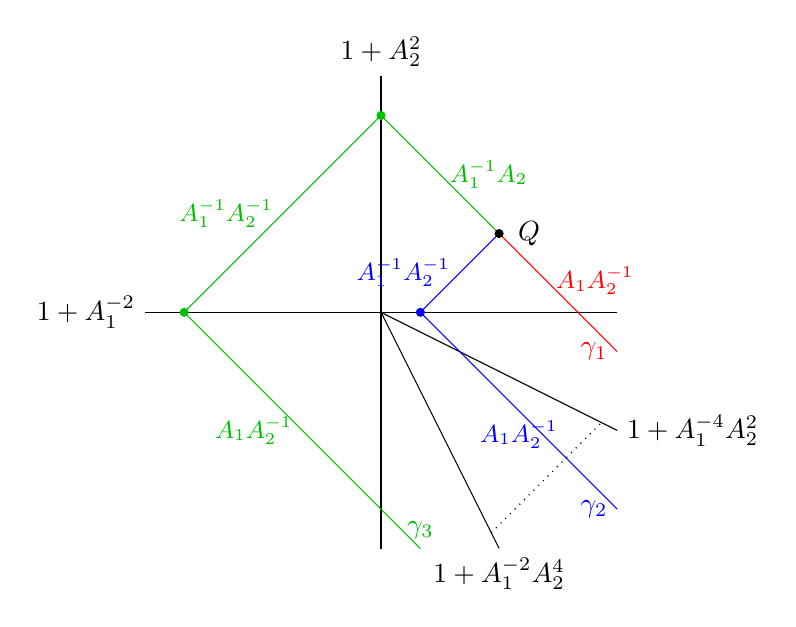
\begin{tikzpicture}
    \draw (3,0) -- (-3,0) node[left] {$1+A_1^{-2}$};
    \draw (0,-3) -- (0,3) node[above] {$1+A_2^2$};
    \draw (0,0) -- (3,-1.5) node[right] {$1+A_1^{-4}A_2^2$};
    \draw (0,0) -- (1.5,-3) node[below] {$1+A_1^{-2}A_2^4$};
    \draw (1.5,1) node[circle, right] {$Q$};
    \draw[dotted] (1.4,-2.8) -- (2.8,-1.4);
    \draw[red] (3,-0.5) -- (1.5,1);
    \draw[red] (2.1,0.1) node[above right]{\small $A_1 A_2^{-1}$};
    \draw[red] (3,-0.5) node[left]{$\gamma_1$};
    \draw[blue] (0.5,0) -- node[left] {\small $A_1^{-1} A_2^{-1}$}  (1.5,1);
    \draw[blue] (0.5,0) -- node[below] {\small $A_1 A_2^{-1}$} (3,-2.5);
    \draw[blue] (3,-2.5) node[left]{$\gamma_2$};
    \draw[green!75!black] (0,2.5)  -- node[right] {\small $A_1^{-1}A_2$} (1.5,1);
    \draw[green!75!black] (-2.5,0) -- node[left] {\small $A_1^{-1} A_2^{-1}$}  (0,2.5);
    \draw[green!75!black] (0.5, -3)  --node[left] {\small $A_1 A_2^{-1}$} (-2.5,0);
    \draw[green!75!black] (0.5,-3) node[above]{$\gamma_3$};
    \draw[color=blue,fill=blue] (0.5,0) circle (0.5mm);
    \draw[color=green!75!black,fill=green!75!black] (0,2.5) circle (0.5mm);
    \draw[color=green!75!black,fill=green!75!black] (-2.5,0) circle (0.5mm);
    \draw[color=black,fill=black] (1.5,1) circle (0.5mm);
  \end{tikzpicture}
  \caption{Example~\ref{brokenex}} 
  \label{figbrokenex}
\end{figure}

The following summarizes the main properties of the theta functions as shown in
\cite{GHKK}:
\begin{theorem} $ $
  \begin{enumerate}
    \item
      If $\fD$ is any consistent scattering diagram, $Q$, $Q'$ are two general
      irrational points on $M_{\RR} \backslash$ Supp$(\fD)$, and $\gamma$ is a
      path joining $Q$ to $Q'$, then 
      \[
        \theta_{\gamma, \fD }(\vartheta_{Q,m}) = \vartheta_{Q', m}. 
      \]
    
    \item 
      Taking $\fD=\fD_{(b,c)}$, if $Q$ lies in the interior of a chamber of
      $\fD$, then $\vartheta_{Q,m}$ is a Laurent polynomial for any $m$.
    
    \item 
      Taking $\fD=\fD_{(b,c)}$, if $Q$ lies in the interior of the first
      quadrant, then $\vartheta_{Q,m}$ is a universal Laurent polynomial for
      any $m$.

    \item 
      Taking $\fD=\fD_{(b,c)}$, if $m$ lies in the interior of a chamber of
      $\fD$, and $Q$ lies in the same chamber, then $\vartheta_{Q,m}=A^{m}$.
   
  \end{enumerate}
\end{theorem}

\begin{proof}
  (1) is a main result of \cite{CPS}, quoted in this context in \cite{GHKK},
  Theorem 3.5.  The second statement is \cite{GHKK}, Example 7.18: there,
  $\Theta$ is the subset of $M$ consisting of those $m$ for which
  $\vartheta_{Q,m}$ is a Laurent polynomial for $Q$ in the interior of 
  some chamber of $\fD$ (and hence by \cite{GHKK}, Proposition 7.1, all 
  chambers).
  Next, (3) follows from (2) by Theorem \ref{univLaurent}. 
  Finally, (4) follows from \cite{GHKK}, Proposition 3.8 (use the argument of
  \cite{GHKK}, Theorem 4.8 in the case that the chamber is not the positive
  quadrant.)
\end{proof}

\begin{remark} 
  \label{rk:theta functions g-vector}
  If $m\in M$ lies in one of the chambers of $\fD_{(b,c)}$, and $Q$ lies in
  the first quadrant, then from (1) and (4) of the above theorem,
  $\vartheta_{Q,m}=\theta_{\gamma,\fD_{(b,c)}}(A^{m})$ for a path $\gamma$
  joining the chamber containing $m$ to $Q$. Moreover it follows from the
  details of the proof of Theorem \ref{univLaurent} that $\vartheta_{Q,m}$ is
  a cluster monomial, and from \cite{GHKK}, Theorem 7.5, that the 
  ${\bf g}$-vector of this cluster monomial is precisely $m$. 
\end{remark}

\begin{example}
  Let us try one more calculation with broken lines. We take the same scattering
  diagram as in example~\ref{brokenex}. Now take the initial momentum $m=(2,-2)$
  with the same endpoint $Q$. By similar calculations we get 
  \[ 
    \vartheta _{Q, (2,-2)} = 
    A_1^2 A_2^{-2} + A_1^{-2}A_2^2 + A_1^{-2}A_2^{-2} + 2 A_2^{-2} + 2A_1^{-2}.  
  \]
  Note that 
  \[ 
    \vartheta _{Q, (2,-2)} = 
    \left(\vartheta_{Q, (1,-1)}\right) ^2 -2. 
  \]
  In this scattering diagram $\fD_{(2,2)}$, the ray with momentum $(1,-1)$ does
  not lie in the interior of any chamber. So neither $\vartheta_{Q,(1,-1)}$ nor 
  $\vartheta _{Q, (2,-2)}$ are cluster monomials.

  There are a number of known bases for $\cA(2,2)$, which give different results
  for the basis elements with ${\bf g}$-vectors $(d,-d)$ for $d>0$. Our
  calculations shows that at least for $d=1$ or $2$, theta functions agree with
  the greedy basis elements.
\end{example}


\section{Relation to greedy bases}
\saySS{At a certain point in our discussion in Snowbird we decided we were going
  to use the scattering diagram $\fD_{\mathrm{gr},(b,c)}$ instead of
  $-\fD_{\mathrm{gr},(b,c)}$ because we would have the base point $Q$ in the
  first quadrant and most of the rays in the third one. By doing so we get that
  theta functions in $\fD_{\mathrm{gr},(b,c)}$ are parametrized by the
  \emph{negative} of their ${\bf d}$-vectors. On the other hand, in
  $\fD_{(b,c)}$ theta functions are parametrized by their ${\bf g}$-vectors.
  This is slightly counterintuitive, maybe it is  more natural to change
  our convention.}
\sayMG{I would be slightly inclined to stick with the convention we
  are currently using in the paper, as it is a less drastic change
  from what is used in GHKK}
As mentioned in Remark \ref{rk:theta functions g-vector}, theta functions are
parametrized by their ${\bf g}$-vectors. On the other hand the description of
greedy elements given in \cite{LLZ} is in terms of their ${\bf d}$-vectors (cf.
Remark 1.9 ibid.). 

In order to compare the two we will leverage the observation that, in rank 2,
these families of vectors are related by an easy piecewise-linear transformation
as explained in the paragraph following Conjecture 3.21 in \cite{RS}. We will do
so via a scattering diagram $\fD_{\mathrm{gr},(b,c)}$ closely related to
$\fD_{(b,c)}$.

Let $T:M_\RR\rightarrow M_\RR$ be the piecewise-linear map given by
\[
  T (m) := 
  \begin{cases}
    m   & m_2 \geq 0 \\
    m + (bm_2,0), & m_2 \leq 0.
  \end{cases}
\]
We will denote its domains of linearity by 
\[ 
  \mathcal{H}_{+} := 
  \left\{ m \in M_{\mathbb{R}}\, |\, m_2 \geq 0 \right\} 
  \quad
  \mbox{and}
  \quad
  \mathcal{H}_{-} := 
  \left\{ m \in M_{\mathbb{R}} \,|\, m_2 \leq 0 \right\}.
\]
Let $T_+$ and $T_-$ be the linear extensions to $M_\RR$ of $T|_{\mathcal{H}_+}$
and $T|_{\mathcal{H}_-}$ respectively ($T_+$ is just the identity map but it
will be convenient to use this notation in what follows). 
By (\ref{eqn:linear action}) both $T_+$ and $T_-$ act on pairs $(\fd,f_\fd)$ so
we can use them to define the image of such pairs under $T$. Namely set
\[
  T(\fd,f_\fd):=
  \left\{
    T_+\left(\fd\cap\mathcal{H}_+,f_\fd\right),
    T_-\left(\fd\cap\mathcal{H}_-,f_\fd\right)
  \right\}.
\]

Having fixed the notation we are ready to introduce $\fD_{\mathrm{gr},(b,c)}$.
The set
\[
  T(\fD_{(b,c)}):=
  \left\{
    T(\fd,f_\fd)\, |\, (\fd,f_\fd)\in \fD_{(b,c)}
  \right\}
\]
is not a scattering diagram according to Definition 
\ref{def:scattering_diagram} (not all of its elements are walls for the same
convex cone) but can be made into one by few quick fixes.

First of all $\big( \RR (0,1), 1+A_2^c\big)$ is the only wall of $\fD_{(b,c)}$
whose support is not totally contained in one of the domains of linearity of
$T$; therefore, under $T$, it breaks into two parts:
\[
  \big( \RR_{\ge0} (0,1), 1+A_2^c\big)
  \quad
  \mbox{and}
  \quad
  \big( \RR_{\le 0} (b,1), 1+A_1^{bc}A_2^c\big).
\]

Next note that, since $T(-1,0)=(-1,0)$ and $T(b,-1)=(0,-1)$, $T$ maps all the
walls of $\fD_{(b,c)}\setminus\fD_{\mathrm{in},(b,c)}$ to the third quadrant. 
Indeed 
\[
  \big(\RR_{\leq0}(-b,1),1+A_1^{-bc}A_2^c\big)
\]
is the wall with the biggest slope in
$\fD_{(b,c)}\setminus\fD_{\mathrm{in},(b,c)}$ and its image is 
\[
  \big( \RR_{\le0} (0,1), 1+A_2^c\big).
\]

\begin{defn}
  $\fD_{\gr,(b,c)}$ is the scattering diagram obtained from
  $T\left(\fD_{(b,c)}\right)$ by replacing 
  \begin{itemize}
    \item
      $\big(\RR (-1,0), 1+A_1^{-b}\big)$ with $\big(\RR  (1,0), 1+A_1^b\big)$,
    \item 
      both $ \big( \RR_{\ge0} (0,1), 1+A_2^c\big)$ and $\big( \RR_{\le0} (0,1),
      1+A_2^c\big)$ with $ \big( \RR (0,1), 1+A_2^c\big)$.
  \end{itemize}
  Its base region is the cone $\sigma_\gr$ generated by $(1,0)$ and $(0,1)$.
\end{defn}

\begin{remark}
  It is not too hard to see that the scattering diagram $\fD_{\gr,(b,c)}$ is
  consistent. This fact, together with the uniqueness property implied by
  \cite[Theorem 1.7]{GHKK}, gives an alternative way to introduce it. Indeed, in
  analogy with the definition of $\fD_{(b,c)}$, one could consider the
  scattering diagram
  $\fD_{\gr,\mathrm{in},(b,c)}$ given by 
  \[
    \fD_{\gr,\mathrm{in},(b,c)}=
    \left\{
      \big(\RR (1,0), 1+A_1^b\big), 
      \big(\RR (0,1), 1+A_2^c\big)
    \right\}
  \]
  and obtain $\fD_{\gr,(b,c)}$ using Theorem \ref{KS}. 
\end{remark}

For a broken line $\gamma$ in $\fD_{(b,c)}$, we denote its image under $T$ as
$T(\gamma)$: this is the broken line in $\fD_{\gr,(b,c)}$ whose underlying map
is $\gamma\circ T$. Given any domain of linearity $L$ of $\gamma$, by
subdividing it when necessary, we can always assume that either $\gamma(L)
\subset \mathcal{H}_{+} $ or $\gamma(L)\subset \mathcal{H}_{-}$. The monomial
attached to $L$ in $T(\gamma)$ is then obtained by applying, accordingly, either
$T_+$ or $T_-$ to the exponent of the monomial attached to $L$ in $\gamma$.

\begin{theorem}
  \label{thm:T_on_broken_lines}
  The map $T$ defines a one-to-one correspondence between broken lines in $\fD_{(b,c)}$
  for $m$ with endpoint $Q$ and broken lines in $\fD_{\gr,(b,c)}$ for $T(m)$
  with endpoint $T(Q)$. In particular for $Q \in \mathcal{H}_+$ or $\mathcal{H}_-$,
  we have
  \[ 
    \vartheta^{\gr}_{T(Q),T( m)} = 
    T_{+} \left(\vartheta_{Q, m}\right) 
    \quad
    \mbox{or} 
    \quad
    T_{-} \left(\vartheta_{Q, m}\right)
  \]
  respectively.
\end{theorem}

\begin{proof}
  This is essentially the same as the argument of \cite{GHKK}, Prop.\ 3.6.  To
  prove the statement, we only need to check the bending at the $x$-axis. Let
  $L$, $L'$ be the domains of linearity of $\gamma$ before and after bending
  along $\RR (-1,0)$. So $c(L') A^{m(L')}$ is a term in 
  \[
    \theta_{-m(L),\RR(-1,0)} \left(c(L) A^{m(L)}\right)
    = 
    c(L) A^{m(L)} \left(1+A_1^{-b}\right) ^{|m_2(L)|}.
  \]

  First, assume $\gamma$ passes from $\mathcal{H}_-$ to $\mathcal{H}_+$. In this
  case, we have $m_2(L) < 0$. Now in order for the monomial
  $c(L')A^{T_+(m(L'))} =c(L')A^{m(L')}$ attached to $L'$ in
  $T\circ\gamma$ to satisfy the bending rule, it must be a term in
  \[
    \theta_{-T_-(m(L)),\RR (1,0)} \left(c(L) A^{T_-(m(L))}\right). 
  \]
  Since the second component of $T_-(m(L))$ is $m_2(L)$ we get
  \begin{align*} 
    \theta_{-T_-(m(L)),\RR (1,0)} \left(c(L) A^{T_-(m(L))}\right) 
    & =
    c(L) A^{T_-(m(L))} \left(1+A_1^b\right) ^{-m_2(L)}
    \\
    & = 
    c(L) A^{m(L)} A_1^{b m_2(L)} 
    \left(1+A_1^b\right)^{-m_2(L)} 
    \\
    & = 
    c(L) A^{m(L)} \left(1+A_1^{-b}\right) ^{-m_1(L)}.
  \end{align*}
  This shows that $T_k(\gamma)$ satisfies the correct rule when bending along
  $(\RR (1,0), 1+A_1^b)$ if $\gamma$ passes from $\mathcal{H}_-$ to
  $\mathcal{H}_+$. By repeating similar calculations, we can see that this also
  holds when $\gamma$ passes from $\mathcal{H}_+$ to $\mathcal{H}_-$.
\end{proof}

The following demonstrates the utility of using $\fD_{\gr,(b,c)}$:

\begin{prop}
  For any  $m\in M$, if $Q$ lies in the first quadrant, then 
  \[
    \vartheta^{\gr}_{Q, m}=A^{m}\left(1+f(A_1,A_2)\right)
  \]
  where $f\in (A_1,A_2)\subseteq \Bbbk[A_1,A_2]$.
  In particular, $m$ is the negative of the ${\bf d}$-vector of
  $\vartheta^{\gr}_{Q,m}$.
\end{prop}

\begin{proof}
  For any $m\in M$ and any $Q$ in the first quadrant, there is always a broken
  line $\gamma$ for $m$ and $Q$ that does not bend at any wall. Therefore $\Mono
  (\gamma) = A^{m}$ always appears as a term in $\vartheta^{\gr}_{Q,m}$.

  However, because the functions attached to the walls of
  $\fD_{\gr,(b,c)}$ are all of the form $1+g(A_1,A_2)$ with $g(A_1,A_2) \in
  (A_1,A_2) \subseteq \Bbbk[[A_1,A_2]]$, it follows that any term coming from a
  broken line which bends must be of the form $cA^{m}A_1^{d_1}A_2^{d_2}$ with
  $d_1,d_2\ge 0$, $d_1+d_2>0$. This proves the result.
\end{proof}

\sayMG{It might be appropriate to add stuff about the quantum version here.
  Right now I don't know if we can easily prove enough facts about the quantum
  version for our main result. I suggest we wait until the rest is written up
  and then I see whether it is possible to extend the proof given what we
  currently know. (For example, in general I don't know how to get the chamber
  structure that is visible in the classical case.)}

\begin{remark}
  Combining Theorem \ref{thm:T_on_broken_lines} with the above result, when $Q$
  is in the first quadrant we obtain the parametrization of
  theta functions we were after. Indeed we get 
  \[
    \vartheta^\gr_{Q,T(m)}=\vartheta_{Q,m}
  \]
  with $m$ being its ${\bf g}$-vector and $T(m)$ the negative of its 
  ${\bf d}$-vector.
\end{remark}
\saySS{Eventually we want to make a saner version of the bibliography; this is
  kind of an hack.}

\section{Proof that the bases coincide}

We may now state the main theorem in our current notation.

\begin{thm}
For any integers $b,c>0$ and for each $(m_1,m_2)\in \mathbb{Z}^2$, we have that 
\[ \Theta_{(m_1,m_2)} = x[?,?]\]
as elements in the cluster algebra $\mathcal{A}(b,c)$.  Hence, the greedy basis and the theta basis for $\mathcal{A}(b,c)$ coincide.
\end{thm}

The proof will be to show that $\Theta_{(m_1,m_2)}$ is a pointed element with the same Newton polytope as $x[?,?]$.  By Theorem \ref{thm:  ???}, this is already enough to show that $\Theta_{(m_1,m_2)}=x[?,?]$.

Let $\Gamma$ be a broken line in $\mathfrak{D}_{(b,c)}$.  At any point $Q=(q_1,q_2)\in \Gamma$ at which $\Gamma$ is linear with momentum $m=(m_1,m_2)$, define the \emph{angular momentum} of $\Gamma$ at $Q$ to be $q_1m_2-q_2m_1$.

\begin{lemma}
The angular momentum is constant on $\gamma$.
\end{lemma}
\begin{proof}
Let $q$ and $q'$ be two points on $\gamma$.
First, assume that $q=(q_1,q_2)$ and $q'=(q_1',q_2')$ are in the same linear region of $\gamma$, with momentum $m=(m_1,m_2)$.  There is some $t$ such that 
\[ (q_1',q_2') = (q_1+tm_1,q_2+tm_2) \]
Then the angular momentum at $q'$ is 
\[ (q_1+tm_1)m_2-(q_2+tm_2)m_1 = q_1m_2 - q_2m_1 \]

Next, assume that $q$ and $q'$ are points on $\gamma$ on either side of a bend at a wall $(\fd, f_{\fd})$ at point $q''=(q_1'',q_2'')$.  If the momentum of $\gamma$ is $m=(m_1,m_2)$ and $f_{\fd}$ is a series in $A^{(w_1,w_2)}$, then the momentum of $\gamma$ at $q'$ must be of the form $(m_1+kw_1,m_2+kw_2)$ for some positive integer $k$.  By the argument of the previous paragraph, the angular momentum at $q$ is $q_1''m_2-q_2''m_1$
and the angular momentum at $q'$ is
\[ q_1''(m_2+iw_2)-q_2''(m_1+iw_1) = (q_1''m_2-q_2''m_1)+k(q_1''w_2-q_2''w_1) \]
Since the point $(q_1'',q_2'')$ lies on the ray through $(w_1,w_2)$, the expression $q_1''w_2-q_2''w_1$ is zero, and so the angular momenta at $q$ and $q'$ are the same.  This equality extends transitively to any pair of points $q,q'$ on $\gamma$.
\end{proof}
The sign of the angular momentum is a useful invariant for characterizing the qualitative behavior of a broken line.
For a broken line ending in the first quadrant, the sign of the angular momentum characterizes whether that broken line could have passed through the fourth quadrant (positive) or the second quadrant (negative).

\begin{lemma}
Let $\gamma$ be a broken line $\mathfrak{D}_{gr,(b,c)}$ with endpoint $q$ in the first quadrant. If $\gamma$ has positive (respectively, negative) angular momentum, then the slope of the linear domains of $\gamma$ decreases (resp. increases) at each bend, except possibly at the boundary of the first quadrant. 
%\begin{itemize}	
	%\item If $\gamma$ has positive angular momentum, then the slope of the linear domains of $\gamma$ decreases at each bend, except possibly at the boundary of the first quadrant.
	%\item If $\gamma$ has negative angular momentum, then the slope of the linear domains of $\gamma$ increases at each bend, except possibly at the boundary of the first quadrant.
%\end{itemize}
\end{lemma}

\tikzstyle{wall}=[draw=black!25,thick]
\tikzstyle{dot} = [blue,fill=blue,inner sep=0.25mm,circle,draw,minimum size=.5mm]

\noindent Figure \ref{fig: brokenlineexample} depicts a broken line with positive angular momentum.  The slopes of the linear domains decreases from $\frac{5}{4}$ to $1$ to $\frac{1}{2}$ before increasing to $+\infty$.

\begin{figure}[h!t]
\begin{tikzpicture}
    \begin{scope}[scale=.75]
    	\clip (-5.5,-5.5) rectangle (5.5,5.5);
    	%\draw[step=1,draw=black!10,very thin] (-10,-10) grid (10,10);
        \draw[wall] (0,0) to (0,10);
        \draw[wall] (0,0) to (-10,0);
        
        \draw[wall] (0,0) to (-12,-6);
        \draw[wall] (0,0) to (-12,-8);
        \draw[wall] (0,0) to (-12,-9);
        \draw[wall] (0,0) to (-12,-9.6);
        \draw[wall] (0,0) to (-12,-10);
        \draw[wall] (0,0) to (-12,-10.28);
        \draw[wall] (0,0) to (-6,-12);
        \draw[wall] (0,0) to (-9,-12);
        \draw[wall] (0,0) to (-9.6,-12);
        \draw[wall] (0,0) to (-10,-12);
        \draw[wall] (0,0) to (-10.28,-12);        
        \path[fill=black!25] (0,0) to (-10.5,-12) to (-12,-10.5) to (0,0);
        \draw[wall, draw=red!25] (0,0) to (-10,-10);
        \draw[wall,black] (0,0) to (10,0);
        \draw[wall,black] (0,0) to (0,-10);
        \draw[wall,black] (0,0) to (-8,-12);
				
			  \draw[blue,thick] (2,1.73) to node[right] {$m=(0,1)$} (2,0) to node[below right] {$m=(2,1)$} (0,-1) to node[below right] {$m=(2,2)$} (-2,-3) to node[right] {$m=(4,5)$} (-6,-7);
				\node[dot] at (2,0) {};
				\node[dot] at (0,-1) {};
				\node[dot] at (-2,-3) {};
				\node[dot,draw=black, fill=black] (q) at (2,1.73) {};
				\node[above right] at (q) {$q$};
				
				\node[below left,black!25] at (5.5,5.5) {Quadrant I};
				\node[below right,black!25] at (-5.5,5.5) {Quadrant II};
				\node[above left,black!25] at (5.5,-5.5) {Quadrant IV};
				
    \end{scope}
\end{tikzpicture}
\caption{A broken line with positive angular momentum}
\label{fig: brokenlineexample}
\end{figure}

\begin{proof}
The lemma is straightforward except for broken lines with initial momentum $(m_1,m_2)$ with $m_1,m_2>0$.  
Consider a bend of $\gamma$ at a point $(q_1,q_2)$ in a wall $(\fd,f_{\fd}(A^{(w_1,w_2})))$.  If the momentum immediately before the bend is $(m_1,m_2)$, the momentum immediately after the bend is $(m_1-kw_1,m_2-kw_2)$ for some positive integer $k$.  

Assume that $(q_1,q_2)$ is not in the boundary of the first quadrant, so that $(q_1,q_2)$ is a negative scalar multiple of the exponent vector $(w_1,w_2)$. If the angular momentum $q_1m_2-q_2m_1$ is positive, then the cross-product $w_1m_2-w_2m_1$ is negative. 
\[ w_1m_2-w_2m_1=m_1(m_2-kw_2)-m_2(m_1-kw_1)<0 \Rightarrow \frac{m_2-kw_2}{m_1-kw_1} < \frac{m_2}{m_1}\]
If the angular momentum is negative, the slope increases by the same argument.
\end{proof}

We can now constrain the possible final momentum of a broken line, which will be used to bound the Newton polytope of the corresponding theta function.

\begin{lemma}
Let $\gamma$ be a broken line in $\mathfrak{D}_{gr,(b,c)}$ which begins in the third quadrant, with endpoint $q$ in the first quadrant.  Denote the  initial momentum by $m=(m_1,m_2)$ and the final momentum by $m^q=(m_1^q,m_2^q)$.  
\begin{enumerate}
	%\item $m_1-m_1^q\in b\mathbb{N}$ and $m_2-m_2^q\in c\mathbb{N}$.%\footnote{Are the $b$ and $c$ correct here?}
	\item If $\gamma$ has positive angular momentum, then $m_2\geq m_2^q>0$ and
	\[ m_1\geq m_1^q\geq\left( \frac{m_1}{m_2}-b\right)m_2^q\]
	where the lower bound is equality only when $m^q =( m_1-bm_2,m_2)$.
	\item If $\gamma$ has negative angular momentum, then $m_1\geq  m_1^q>0$ and
	\[ m_2 \geq m_2^q\geq\left( \frac{m_2}{m_1}-c\right)m_1^q\]
	where the lower bound is equality only when $m^q =( m_1,m_2-cm_1)$.
\end{enumerate}
\end{lemma}
\begin{proof}
Assume $\gamma$ has positive angular momentum; consequently, $\gamma$ passes through the fourth quadrant before entering the first quadrant.  Let $(m_1',m_2')$ be the momentum on $\gamma$ in the fourth quadrant.  By the preceding lemma, $\frac{m_2'}{m_1'}\leq \frac{m_2}{m_1}$ with equality only if $\gamma$ doesn't bend before it reaches the fourth quadrant.  

As the broken line passes into the first quadrant, it may bend at the wall $(\mathbb{R}(1,0),1+A^{(b,0)})$.  By definition, the momentum on $\gamma$ in the first quadrant must be an exponent that appears in $A^{(-m_1',-m_2')}(1+A^{(b,0)})^{m_2'}$.  It follows that%The possible monomials which may occur in this expression are of the form $A^{(-m_1'+kb,-m_2')}$ for some $0\leq k\leq m_2'$, and so 
\[ (m_1^q,m_2^q) = (m_1'-kb,m_2')\]
for some $0\leq k\leq m_2'$.
Consequently, $m_2^q=m_2'\geq0$ and 
\[ m_1^q\geq m_1' - bm_2' = \left(\frac{m_1'}{m_2'} - b\right) m_2'  = \left(\frac{m_1'}{m_2'} - b\right) m_2^q \geq \left(\frac{m_1}{m_2} - b\right) m_2^q\]
The second inequality is equality only if $(m_1',m_2')=(m_1,m_2)$, and so the composite inequality is equality only if $m^q =( m_1-bm_2,m_2)$.

Analogous inequalities hold for negative angular momentum by the same argument.
\end{proof}

\begin{proof}[Proof of Theorem \ref{thm: ???}]
TO DO.
\end{proof}
\begin{thebibliography}{99}
  
  \bibitem[CPS]{CPS} M.~Carl, M.~Pumperla, and B.~Siebert, A tropical view of Landau-Ginzburg models, available at http://www.math.uni-hamburg.de/home/siebert/preprints/LGtrop.pdf
  \bibitem[FZ]{FZ} S.~Fomin and A.~Zelevinsky, Cluster algebras I: Foundations,  \textsl{J. Amer. Math. Soc.} \textbf{15} (2002), no. 2, pp.~497--529.
  \bibitem[G10]{G10} M.~Gross,  \emph{Mirror symmetry for $\mathbb{P}^2$ and tropical geometry}, Adv.\ Math., {\bf 224} (2010), 169--245. 
  \bibitem[GHK11]{GHK11} M.~Gross, P.~Hacking and S.~Keel, \emph{Mirror symmetry for log Calabi-Yau surfaces I}, preprint, 2011.
  \bibitem[GHKK]{GHKK} M.~Gross, P.~Hacking, S.~Keel, M.~Kontsevich, \emph{Canonical bases for cluster algebras}, preprint, 2014.
  \bibitem[IOTW]{IOTW} K.~Igusa, K.~Orr, G.~Todorov, J.~Weyman \emph{Picture groups of finite type and cohomology in type $A_n$}, preprint, available at http://people.brandeis.edu/~igusa/Papers/PictureGroup.pdf 
  \bibitem[LLZ2]{LLZ2} K. Lee, L. Li and A. Zelevinsky, Positivity and tameness in rank 2 cluster algebras, \textsl{J. Alg. Comb.} 2014, doi: 10.1007/s10801-014-0509-6.
  \bibitem[LLZ]{LLZ} K.~Lee, L.~Li, and A.~Zelevinsky, Greedy elements in rank 2 cluster algebras, \textsl{Selecta Math.} \textbf{20} (2014), 57--82.
  \bibitem[LLZ]{LLZ} K.~Lee, L.~Li, A.~Zelevinsky \emph{Greedy elements in rank 2 cluster algebras}, Selecta Math. (N.S.), {\bf 20}, (2014), 57--82,
  \bibitem[R]{R} N.~Reading, \emph{Universal geometric cluster algebras}, Mathematische Zeitschrift, {\bf 277 } (2014), 499-547.
  \bibitem[RS]{RS} N.~Reading, D.~Speyer, \emph{Combinatorial frameworks for cluster algebras}, preprint, 2011.
  \bibitem[SZ]{SZ} P.~Sherman and A.~Zelevinsky, Positivity and Canonical Bases in Rank 2 Cluster Algebras of Finite and Affine Types, \textsl{Mosc. Math. J.} \textbf{4} (2004), no. 4, 947--974.

\end{thebibliography}

\end{document}
